% \documentclass[aspectratio=169,notes]{beamer}
\documentclass[aspectratio=169]{beamer}
\usetheme[faculty=phil]{fibeamer}
\usepackage{polyglossia}
\setmainlanguage{english} %% main locale instead of `english`, you
%% can typeset the presentation in either Czech or Slovak,
%% respectively.
\setotherlanguages{russian} %% The additional keys allow
%%
%%   \begin{otherlanguage}{czech}   ... \end{otherlanguage}
%%   \begin{otherlanguage}{slovak}  ... \end{otherlanguage}
%%
%% These macros specify information about the presentation
\title[Theoretical Mechanics]{Theoretical Mechanics, Lab 9: DYN COM LINEAR} %% that will be typeset on the
\subtitle{Theorem on the: \\
\quad Motion of the centre of Mass of a system\\
\quad Change of Linear momentum of a system\\ 
         } %% title page.
\author{Oleg Bulichev}
%% These additional packages are used within the document:
\usepackage{ragged2e}  % `\justifying` text
\usepackage{booktabs}  % Tables
\usepackage{tabularx}
\usepackage{tikz}      % Diagrams
\usetikzlibrary{calc, shapes, backgrounds}
\usepackage{amsmath, amssymb}
\usepackage{url}       % `\url`s
\usepackage{listings}  % Code listings
% \usepackage{subfigure}
\usepackage{floatrow}
\usepackage{subcaption}
\usepackage{mathtools}
\usepackage{todonotes}
\usepackage{fontspec}
\usepackage{multicol}
\usepackage{pdfpages}
\usepackage{wrapfig}
\usepackage{animate}
\usepackage{booktabs}
\usepackage{multirow}
% \usepackage{graphicx}
\usepackage{colortbl}
\usepackage{catchfilebetweentags}
\usepackage{makecell}
\graphicspath{{resources/}}
\frenchspacing

\setbeamertemplate{caption}[numbered]
\usetikzlibrary{graphs}

% \usepackage[backend=biber,style=ieee,autocite=footnote]{biblatex}
% \addbibresource{biblio.bib}
% \DefineBibliographyStrings{english}{%
%   bibliography = {References},}

\newcommand{\oleg}[2][] {\todo[color=red, #1] {OLEG:\\ #2}}
\newcommand{\fbckg}[1]{\usebackgroundtemplate{\includegraphics[width=\paperwidth]{#1}}}%frame background

\usepackage[framemethod=TikZ]{mdframed}
\newcommand{\dbox}[1]{
\begin{mdframed}[roundcorner=3pt, backgroundcolor=yellow, linewidth=0]
\vspace{1mm}
{#1}
\vspace{1mm}
\end{mdframed}
}

\begin{document}
\setlength{\abovedisplayskip}{0pt}
\setlength{\belowdisplayskip}{0pt}
\setlength{\abovedisplayshortskip}{0pt}
\setlength{\belowdisplayshortskip}{0pt}

\fbckg{fibeamer/figs/title_page.png}
\frame[c]{\setcounter{framenumber}{0}
    \usebeamerfont{title}%
    \usebeamercolor[fg]{title}%
    \begin{minipage}[b][6.5\baselineskip][b]{\textwidth}%
        \textcolor{black}{\raggedright\inserttitle}
    \end{minipage}
    % \vskip-1.5\baselineskip

    \usebeamerfont{subtitle}%
    \usebeamercolor[fg]{framesubtitle}%
    \begin{minipage}[b][3\baselineskip][b]{\textwidth}
        \raggedright%
        \insertsubtitle%
    \end{minipage}
    \vskip.25\baselineskip
}
%   \frame[c]{\maketitle}

\fbckg{fibeamer/figs/common.png}



\section*{Tasks}

\begin{frame}[t]{Motion of the centre of mass of a system}
\framesubtitle{}
\footnotesize
    \begin{tabular}{>{\centering\arraybackslash} m{1.2cm}|>{\centering\arraybackslash} m{1cm}|>{\centering\arraybackslash} m{4.3cm}|>{\centering\arraybackslash} m{4cm}|>{\centering\arraybackslash} m{1.3cm} } 
        \toprule
        \toprule
       \textbf{ R. O.} & \textbf{Eqn \#} & \textbf{Equations} & \textbf{Applications} & \textbf{Extra Info} \\ 
        \hline
        \ExecuteMetaData[../../dynamics_methods_overview/dynamics_methods_overview]{sndcomlinear}
        \bottomrule
        \bottomrule
        \end{tabular}
\end{frame}
    
    \begin{frame}[t]{Task 1 and 2 (mine)}
    \framesubtitle{}
    \begin{columns}[T,onlytextwidth]
        \begin{column}{0.49\textwidth}
\scriptsize
            A system consist of body $A$ (rectangular) with mass $m_1$ and a body $B$ (ball) with mass $m_2$ which connected to the body $A$ by rotational joint. 
            
            $OB=l=0.2,\ m_1 = 2,\ m_2 = 0.5$.
            \bigskip

            There are 2 tasks:
            \begin{enumerate}
                \item We need to find $S$ (distance), when the body $B$ moved from $I$ position, to $II$ with applied torque $M$.
                \bigskip

                \textit{Answer}: $S = \dfrac{m_2 l}{m_1 + m_2} = 0.04$
                \item We know that $B$ has an angular velocity $\omega = \epsilon t$, where $\epsilon=const$. We have to find a velocity of $A$, when the body $B$ reaches $II$ position. 
            \end{enumerate}
        \end{column}
        \begin{column}{0.49\textwidth}
            \begin{figure}[H]
                \centering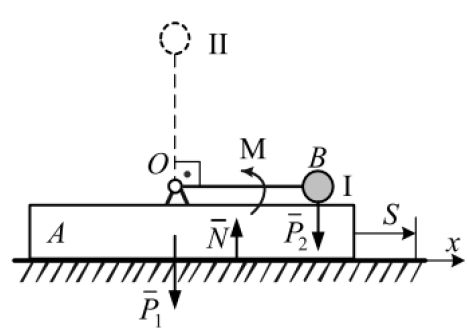
\includegraphics[height=6cm,width=1\textwidth,keepaspectratio]{image6.png}
                \label{fig:image6.png}
            \end{figure}
        \end{column}
    \end{columns}
    \end{frame}
    
    \begin{frame}[t]{Task 3 (yours): M (rus) 35.17}
    \framesubtitle{}
        \begin{figure}[H]
            \flushleft
            \begin{subfigure}{0.59\textwidth}
                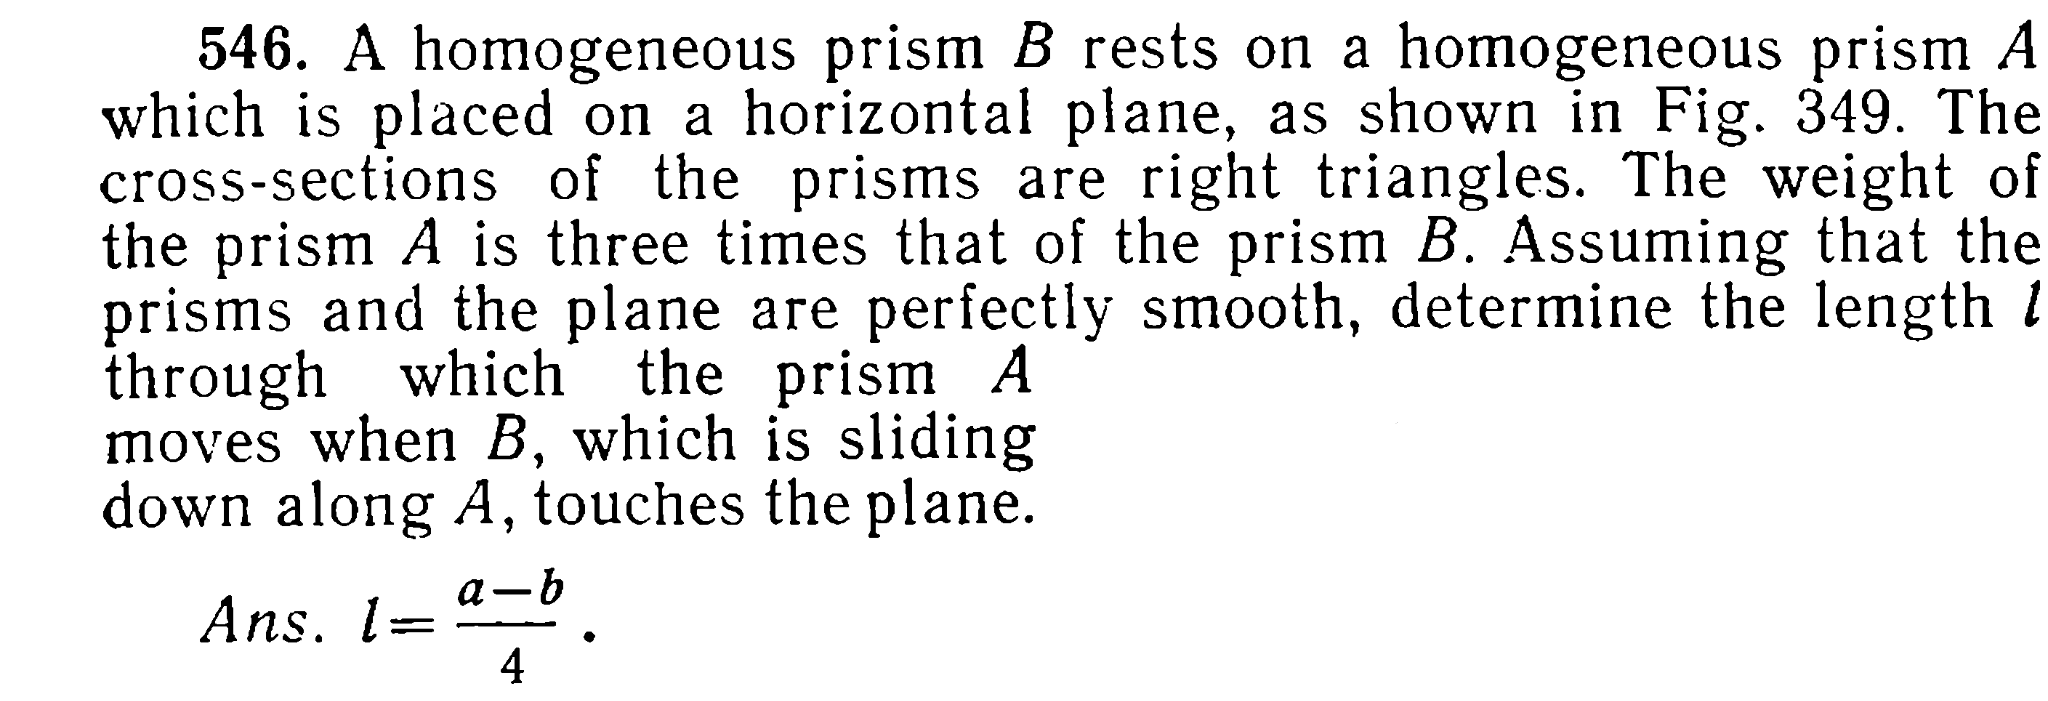
\includegraphics[height=6cm,width=1\textwidth,keepaspectratio]{image10.png}
            \end{subfigure}
            \begin{subfigure}{0.39\textwidth}
                \centering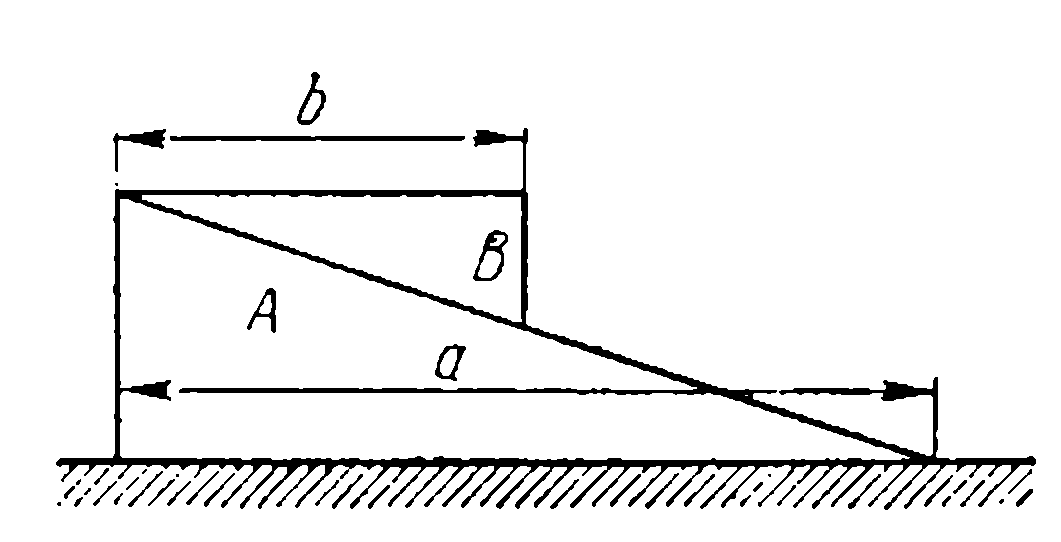
\includegraphics[height=6cm,width=1\textwidth,keepaspectratio]{image9.png}
                \label{fig:image9}
            \end{subfigure}
        \end{figure}
    \end{frame}
    
    \begin{frame}[t]{Task 4 (yours)}
    \framesubtitle{}
        \begin{figure}[H]
            \vspace{-2.0cm}
            \begin{subfigure}{0.69\textwidth}
                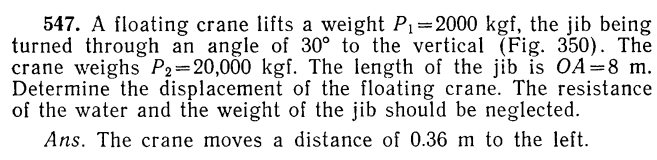
\includegraphics[height=6cm,width=1\textwidth,keepaspectratio]{image13.png}
            \end{subfigure}
            \begin{subfigure}{0.29\textwidth}
                \vspace{2.0cm}
                \centering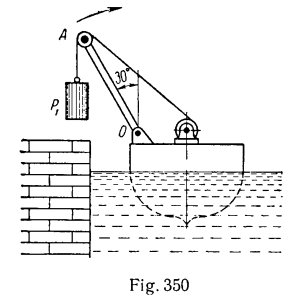
\includegraphics[height=6cm,width=1\textwidth,keepaspectratio]{image8.png}
                % \caption{capture2}
                \label{fig:image8}
            \end{subfigure}
        \end{figure}
    \end{frame}

\fbckg{fibeamer/figs/last_page.png}
\frame[plain]{}
\end{document}